\documentclass[hidelinks,12pt]{article}

\usepackage{amsmath}    % need for subequations
\usepackage{graphicx}   % need for figures
\usepackage{verbatim}   % useful for program listings
\usepackage{color}      % use if color is used in text
\usepackage{subfigure}  % use for side-by-side figures
\usepackage{hyperref}   % use for hypertext links, including those to external documents and URLs

\usepackage[numbered]{matlab-prettifier} % including matlab w/ syntax highlighting
\usepackage[T1]{fontenc} % prettier matlab font
\lstMakeShortInline[style=Matlab-editor]| % matlab inline escape character

\usepackage[
top    = 2.75cm,
bottom = 2.50cm,
left   = 3.00cm,
right  = 2.50cm]{geometry}

\graphicspath{ {./Figures/} }

% don't need the following. simply use defaults
\setlength{\baselineskip}{16.0pt}    % 16 pt usual spacing between lines



\begin{document}
\pagenumbering{gobble}
\begin{center}
  {\huge Homework 5}\\
  \vspace{10px}
  
\includegraphics{Logo} \\
  Date of Submission:\\
  February 25, 2019\\
  \vspace{30px}
  \rule{300px}{0.5px} \\
  Thorne Wolfenbarger \\
  \href{mailto:wolfent1@my.erau.edu}{wolfent1@my.erau.edu} \\
  \vspace{30px}
  Submitted to: \\
  Professor Kaela Martin \\
  College of Engineering \\
  \vspace{40px}
  In Partial Fulfillment \\
  of the Requirements of \\
  \vspace{10px}
  AE 313 \\
  Space Mechanics \\
  Spring, 2019 \\
\end{center}

\pagenumbering{arabic}
\begin{center}
\large AE 313 Homework 8
\end{center}
\flushleft
1. Express $\Delta \vec{v}$ in rotating orbit unit vectors $\hat{r}, \hat{\theta} \hat{h}$ as well as inertial unit vectors $\hat{x}, \hat{y}, \hat{z}$.\\
\begin{lstlisting}[frame=lines,style=Matlab-editor,basicstyle = \mlttfamily]
vdv_rth = dv*[cosd(beta)*sind(phi) cosd(beta)*cosd(phi) sind(beta)]';
vdv_eci = rot_rth_eci(RAANm, incm, AOLm) * vdv_rth;
\end{lstlisting}
\begin{tabular}{rl}
  $\Delta \vec{v}_{rth}=$&$<-2.6250,~2.2344,~2.8925> km/s$\\
  $\Delta \vec{v}_{eci}=$&$<3.9498,~-0.8593,~1.9776> km/s$
\end{tabular}\\
\vspace{10px}
2. Determine the position and velocity immediately after the maneuver, $\vec{r}^+, \vec{v}^+$ in the intertial coordinate system.\\
\begin{lstlisting}[frame=lines,style=Matlab-editor,basicstyle = \mlttfamily]
vrp_eci = vrm_eci;
vvp_eci = vvm_eci + vdv_eci;
\end{lstlisting}
\begin{tabular}{rl}
  $\vec{r}^+_{eci}=$&$<-5.9784,~-4.6680,~-0.1583> \cdot 10^3 km$\\
  $\vec{v}^+_{eci}=$&$<11.6963,~-5.4791,~-1.1101> km/s$
\end{tabular}\\
\vspace{10px}
3. Compute the orbital elements $e^+,~i^+,~\Omega^+,~\theta^+,~\theta^{^*+}$ in the new orbit.\\
\begin{lstlisting}[frame=lines,style=Matlab-editor,basicstyle = \mlttfamily]
FPAp = asind(dot(vrp_eci,vvp_eci)/(norm(vrp_eci)*norm(vvp_eci)));
...
true_ap = 360 - true_ap;
\end{lstlisting}
\begin{tabular}{rl}
  $e^+=$ & $2.0151$\\
  $i^+=$ & $6.2208^\circ$\\
  $\Omega^+=$ & $26.9440^\circ$\\
  $\theta^+=$ & $191.1029^\circ$\\
  $\theta^{^*+}=$ & $320.4327^\circ$\\
\end{tabular}\\
\vspace{10px}
4. Find the changes in the elements (including the sign) that occured due to the maneuver, that is, $\Delta e,~\Delta i,~\Delta \Omega,~\Delta \theta$.\\
\begin{lstlisting}[frame=lines,style=Matlab-editor,basicstyle = \mlttfamily]
de = ep-em;
dinc = incp-incm;
dRAAN = RAANp-RAANm;
dAOL = AOLp-AOLm;
\end{lstlisting}
\begin{tabular}{rl}
  $\Delta e=$ & $1.2501$\\
  $\Delta i=$ & $-14.3792^\circ$\\
  $\Delta \Omega=$ & $-7.8560^\circ$\\
  $\Delta \theta=$ & $7.7029^\circ$\\
\end{tabular}\\
\vspace{10px}
5. Confirm the position, $ $m and new orbital elements (problem 3) in GMAT. Plot the original and new orbit (include XY plane and inertial unit vectors). Mark the maneuver location on the plot.\\
\begin{tabular}{rl}
  $\vec{v}^-_{eci}=$&$<7.7465,~-4.6198,~-3.0877> km/s$\\
  $\vec{v}^+_{eci}=$&$<12.026,~-5.1957,~-1.0988> km/s$
\end{tabular}\\
The data in the GMAT orbit is very close to the MATLAB calculations and therefore matches the data from MATLAB calculations.\\
\vspace{10px}
\begin{figure}[!htb]
  \center
  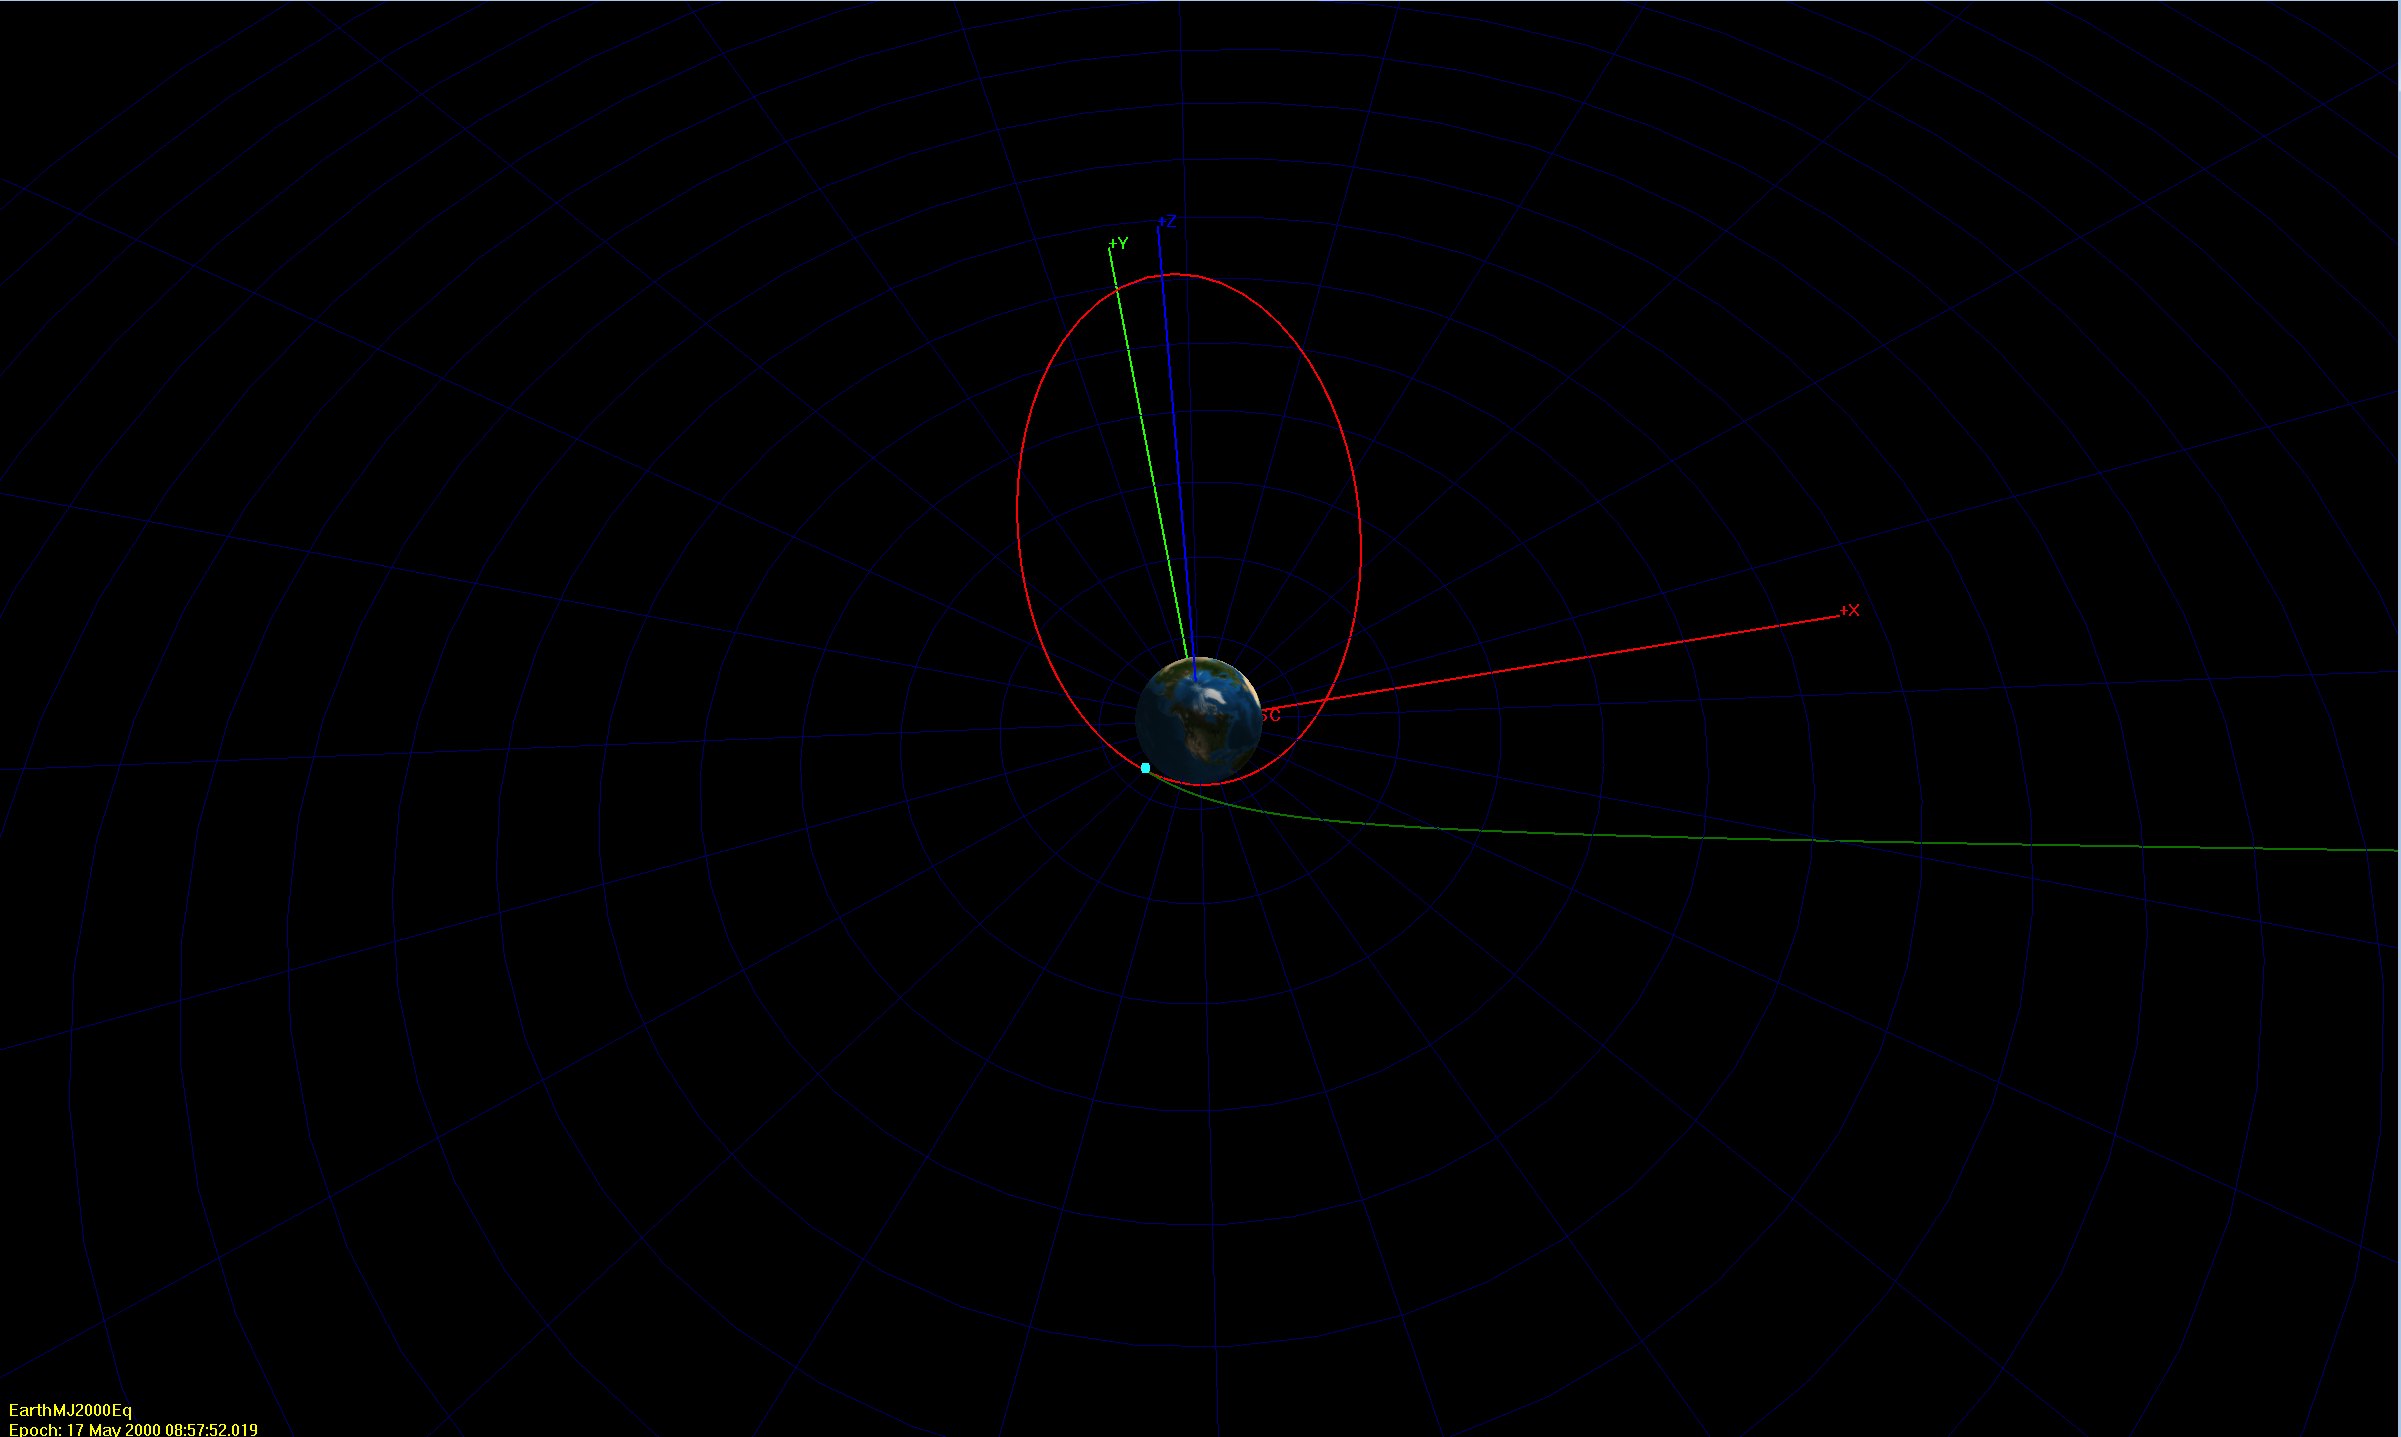
\includegraphics[scale=0.2]{GMAT}
  \caption{GMAT Plot of Orbits}
  \label{fig:temp}
\end{figure}
Turquoise indicates the maneuver point. Clearer view of the maneuver after the code.\\
\vspace{10px}
6. Would you want to perform this maneuver? Why or why not?\\
I would not want to perform this maneuver because it results in a
massively hyperbolic orbit. The goal of the maneuver is to do an orbital
correction, not enter an escape trajectory. With an eccentricity of 2.02,
the orbit is very far from being elliptical.
\begin{tabular}{rl}
\end{tabular}\\
\vspace{10px}
7. Given that the semi-major axes of bi-elliptical transfer are $a_{T1}=6659~km$ and $a_{T2}=6798~km$, what is the departure phase angle? Include a figure/sketch of the phase angle.\\
\begin{lstlisting}[frame=lines,style=Matlab-editor,basicstyle = \mlttfamily]
at1 = 6658;
at2 = 6798;
a_sc = 6378+430;
TOF = pi*(sqrt(at1^3/MU('Earth'))+sqrt(at2^3/MU('Earth')));
n_sc = sqrt(MU('Earth')/a_sc^3);
phase = 2*pi-n_sc*TOF;
phase = phase*180/pi;
\end{lstlisting}
\begin{tabular}{rl}
  $\Delta \Phi=$ & $6.3124^\circ$
\end{tabular}\\
\begin{figure}[!htb]
  \center
  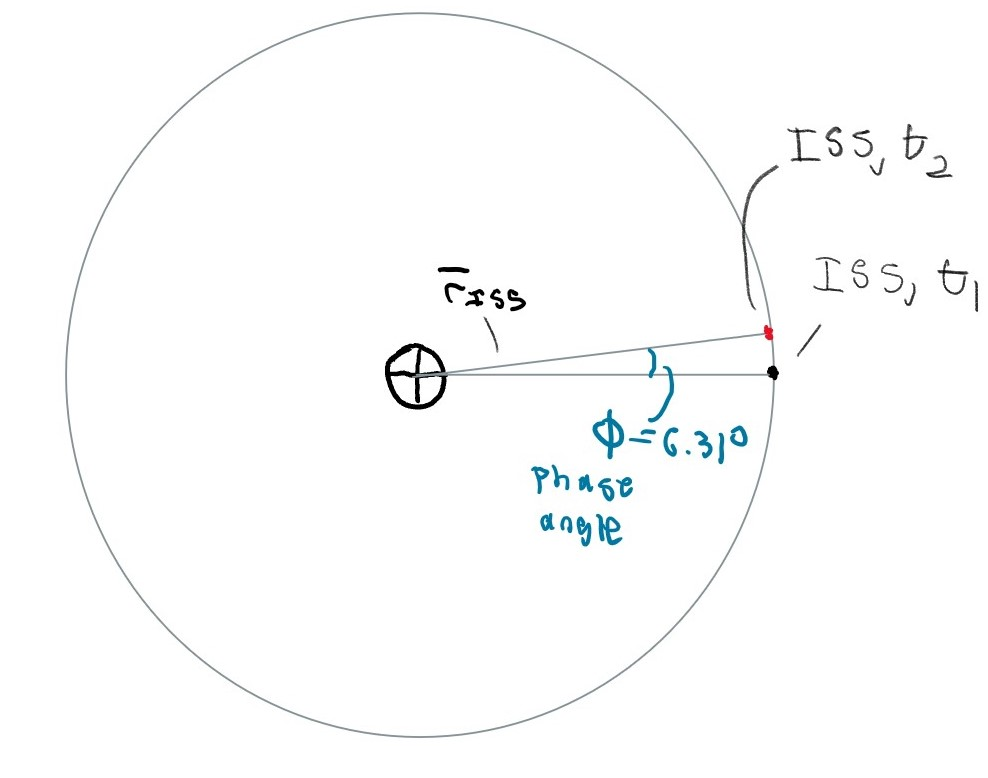
\includegraphics[scale=0.9]{p7}
  \caption{Sketch of the Phase Angle}
  \label{fig:temp}
\end{figure}
\newpage
8. Survey.\\
\begin{figure}[!htb]
  \center
  \includegraphics[scale=0.3]{survey}
  \caption{Survey Screenshot}
  \label{fig:temp}
\end{figure}
\newpage
HW5.m
\begin{lstlisting}[frame=lines,style=Matlab-editor,basicstyle = \mlttfamily]
clc; clear all; close all

%constants
MU = 42828;

% Problem 1
vr = [-2089.6 -2515.7 -6382.0];
vv = [2.1744 0.76911 0.13452];

r = norm(vr)
v = norm(vv)

vh = cross(vr, vv);
h = norm(vh);

syms a
energy_eqn = v^2/2 - MU/r == -MU/(2*a)
energy = v^2/2 - MU/r
a = double(solve(energy_eqn, a))

syms e
h_eqn = h == sqrt(MU*a*(1-e^2))
e = double(solve(h_eqn,e))
e = max(e)

syms E
E_eqn = r == a*(1-e*cos(E));
E = double(solve(E_eqn,E));
E = -min(E) %Because it is descending.

syms time_since_p
time_since_p_eqn = sqrt(MU/a^3)*time_since_p == E - e*sin(E);
time_since_p = double(solve(time_since_p_eqn,time_since_p))

% Problem 2
p = h^2/MU;
true_a = -acos(p/(r*e) - 1/e)
vv_rt = [h*e/p*sin(true_a) h/r 0] % answer

% Problem 3
E1 = E;
t1 = time_since_p;
vr1 = vr;
vv1 = vv;
r1 = r;
v1 = v;
t2 = time_since_p + 12*60*60;
n = sqrt(MU/a^3);
M = n*t2;
E2 = fzero(@(x) x-e*sin(x)-M, 0);
f = 1 - a/r*(1-cos(E2-E1));
g = (t2 - t1) - sqrt(a^3/MU)*(E2 - E1 - sin(E2 - E1));

vr2 = f*vr + g*vv;
r2 = norm(vr2);
fdot = -sqrt(MU*a)/(r2*r1)*sin(E2-E1);
gdot = 1 - a/r2*(1-cos(E2-E1));

vv2 = fdot*vr1 + gdot*vv1 % intertial unit vectors

true_a2 = -acos(p/(r2*e) - 1/e)

vv2_rt = [h*e/p*sin(true_a2) h/r2 0] % radial-tangential

% Problem 4
vr2_peri = [r2*cos(true_a2) r2*sin(true_a2) 0]
vv2_peri = sqrt(MU/p)*[-sin(true_a2) e+cos(true_a2) 0]

% Problem 5

% find i theta omega
syms inc
h_hat = cross(vr2, vv2)/norm(cross(vr2, vv2))
inc_eqn = cos(inc) == dot(h_hat, [0 0 1])
inc = double(solve(inc_eqn,inc))
inc = max(inc)

syms RAAN
RAAN_eqn_1 = sin(RAAN)*sin(inc) == dot(h_hat, [1 0 0])
RAAN_eqn_2 = -cos(RAAN)*sin(inc) == dot(h_hat, [0 1 0])
RAAN1 = double(solve(RAAN_eqn_1));
RAAN2 = double(solve(RAAN_eqn_2));
RAAN = min(RAAN1)*180/pi

syms arg_peri
r1_hat = vr1/norm(vr1)
theta_hat = cross(r1_hat, h_hat)/norm(cross(r1_hat, h_hat))
syms theta
theta_eqn_1 = sin(inc) * sin(theta) == dot(r1_hat, [0 0 1])
theta_eqn_2 = sin(inc) * cos(theta) == dot(theta_hat, [0 0 1])
theta1 = double(solve(theta_eqn_1, theta))
theta2 = double(solve(theta_eqn_2, theta))
theta = intersect(theta1, theta2)
arg_peri_eqn = arg_peri == theta - true_a
arg_peri = double(solve(arg_peri_eqn, arg_peri))
\end{lstlisting}

\newpage
\begin{figure}[!htb]
  \center
  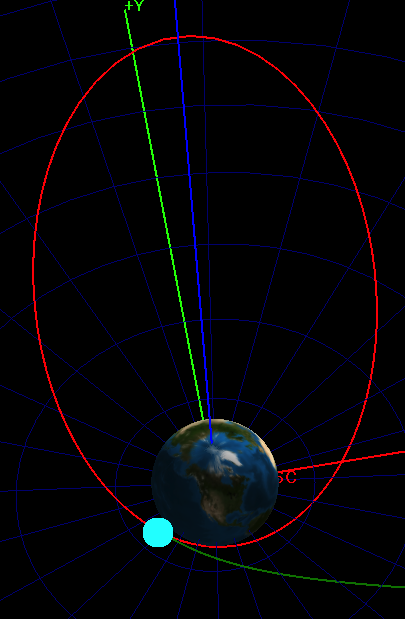
\includegraphics[scale=0.9]{GMAT2}
  \caption{GMAT Modified}
  \label{fig:temp}
\end{figure}
Word has changed their background removal functionality such that I cannot get rid of the black. This is a zoomed photo to help if the first one is difficult to read. Turquoise indicates the maneuver point.
\end{document}
